\documentclass{report}
\usepackage{graphicx}

\setlength{\headsep}{0.0cm}            
\setlength{\headheight}{0.0cm}         
\setlength{\topmargin}{0.0cm}
\setlength{\oddsidemargin}{0.0cm}   
\setlength{\evensidemargin}{0.0cm}  
\setlength{\textwidth}{16.0cm}        
\setlength{\textheight}{24.0cm}
 
\renewcommand{\thesection}{\arabic{section}}

\begin{document}

\hbadness=10000
\hyphenpenalty=10000

\begin{center}
    Vietnam Posts and Telecommunications Institute of Technology (PTIT) \\
    \vspace{0.5cm}
    \Large\textbf{Python 1st Assignment \\ Football Players Statistical Analysis} \\
    \vspace{0.5cm}
    \normalsize 
    Student: Tran, Vu Tien Minh \\
    Student Code: B23DCCE067 \\
    Lecturer: Dr. Kim, Ngoc Bach \\
    Class: D23CQCE04-B \\
    Date: 2025/05/10
\end{center}

\section{Introduction}
This report is the justification and results for the assignment. 
The assignment focuses on collecting and analyzing football players statistical data from 
the 2024-2025 Premier League.

\subsection{The Assignment Tasks}
There are four main tasks:
\begin{enumerate}
    \renewcommand{\labelenumi}{\Roman{enumi}.}
    \item Collecting data from fbref.com for players with more than 90 minutes of 
    playing time.
    \item Statistical calculation by ranking the players, calculating median, mean, standard 
    deviation for each statistic and visualizing the distributions with histograms.
    \item Clustering the players into groups using the K-means algorithm. 
    Reducing the dataset dimention using Principal Component Analysis (PCA) to produce a 2D 
    cluster plot. 
    \item Collecting data from footballtransfers.com. Specifically the transfer value of player 
    with more than 900 minutes of playing time. 
    Choosing a model to estimate transfer value from collected data in task I.
\end{enumerate}

\subsection{Packages Dependencies}
\begin{itemize}
    \item selenium: For getting the page source. Because of acting like a
    browser automator, it can bypass the Cloudflare CAPTCHA and load JavaScript for the 
    complete page source.
    \item beautifulsoup4: For parsing HTML and selecting elements through CSS 
    selector. It is simpler and more powerful compare to selenium's CSS selector.
    \item pandas: For manipulating data. Pandas allows for easy handling and 
    calculation on large datasets. 
    \item matplotlib: For creating visualizations like plots and histograms. 
    It is widely used in data science.
    \item scikit-learn: For data analyzing and predicting players' transfer values. 
    It provides simple and efficient tools and works seemlessly with pandas.
\end{itemize}

\section{Task I: Collecting Data From fbref.com}
The task is to collect all Premier League players specific statistics if they have played for 
mmore than 90 minutes. Each team has its own URL to the statistic tables, there is no URL or 
table which includes all players. The statistics are spread through out many tables.
\begin{verbatim}
    # pseudocode
    players = []
    for team in teams:
        teammates = {}
        for table in team.tables
            for player in table:
                if player.minutes_played > 90:
                    teammates[player.name].extend(player.stats)
        players.extend(teammates.values())
\end{verbatim}

\subsection{Identify The HTML Elements}
The first is begin from the main page and fetch all team URLS from fbref.com
\begin{verbatim}
    <!-- Premier League Table -->
    <table id="results2024-202591_overall">
        <tbody>
            <tr data-row="0">
                <td data-stat="team">
                    <a href="en/squads/822bd0ba/Liverpool-Stats">
                        Liverpool
                    </a>
                </td>
            <tr data-row="1">
                ..
\end{verbatim}
CSS selector to target every \verb|<a>| in the table is:
\begin{verbatim}
    table#results2024-202591_overall > tbody > tr > td[data-stat="team"] > a    
\end{verbatim}

\noindent
Each team's tables source have the same structure:
\begin{verbatim}
    <!-- Liverpool's Standard Stats Table -->
    <table id="stats_standard_9">
        <tbody>
            <tr data-row="0">
                <th>
                    <a>
                        Virgil van Dijk
                    <\a>
                <td data-stat="nationality">...<\td>
                <td data-stat="position">DF<\td>
                <!-- other td -->
            <\tr>
            <!-- other tr from "1" to "24" -->
            <tr class="over_header thead" data-row="25">
                <!-- header info -->
            <\tr>
        <\tbody>
    <\table>
    <!-- other table -->
\end{verbatim}

\noindent
Based on the HTML above, each tr is for one player, each th is the player's name, each td is the 
player's different statistic. But the last tr is just a header, which CSS selector needs to ignore:
\begin{verbatim}
    /* in each table */
    table##{$table-id} > tbody > tr:not(.thead) /* target all tr */ 
    tr > th                                     /* target the th */
    tr > td                                     /* target all td */
\end{verbatim}

\noindent
To select a list of targeted statistics instead of all statistics, the attribute tr.data's 
name need to be checked. The \verb|TABLES_STATS| in \verb|task_i.py| is a list of 
table ids pairing with its statistics. They are used for selecting those targeted statistics list. 
Any unavailable statistic is marked as N/a.

\subsection{Post Processing The Data}
The results will be stored in a pandas.DataFrame and saved to results.csv. However there are issues:
\begin{center}
\centering
    \begin{tabular}{|l|l|l|}
    \hline
    Statistic & Issue & Solution \\
    \hline
    name & duplicate players & keep only the 1st one \\
    \hline
    age & formatted in yy-ddd & calculate the float value \\
    \hline
    minutes & formatted with coma & remove coma \\
    \hline
    nationality & the flag element's text was also scraped & remove flag's text \\
    \hline
    \end{tabular}
\end{center}
Finally, all numeric statistics can now be converted to number, categorical statistics to string, and
missing statistics to N/a

\section{Task II: Statistical Analysis and Visualization}
The assignment further requires analyzing the collected data as follows:
\begin{enumerate}
    \item \textbf{Ranking:} Identify the top 3 and bottom 3 players for each statistic. 
    The results are saved in \verb|top_3.txt|.
    \item \textbf{Statistical Summaries:} For each statistic, calculate the mean, median ans 
    standard deviation across all players and by team. The results are saved in \verb|results2.csv|
    \item \textbf{Histograms:} A histogram is plotted for 3 offensive and 3 defensive statistics
    (the task was updated by the lecturer) to visualize distribution patterns. \verb|matplotlib|
    hist function is used and the results are saved in \verb|histogram\*.html|
    \item \textbf{Best Team:} The team with the highest scores in each statistic is identified. 
    From there, identify the best performing team of the season.
\end{enumerate}

\subsection{Ranking Players}
The task is fairly straight forward. For each DataFrame colums:
\begin{verbatim}
    pandas.Series().nlargest(3) 
    pandas.Series().nsmallest(3) 
\end{verbatim}
This data is crucial for seeing if there are any outliers or extreme values in the features, which
would then be considered later on in the task III and IV.

\subsection{Statistical Summaries}
The mean formula: 
\[Mean = \frac{1}{N} \sum_{i=1}^{N} x_i\]
The median formula: 
\[Median = x_{\left(\frac{N+1}{2}\right)} \quad \textit{(for sorted x)}\]
The standard deviation formula: 
\[\textit{Standard Deviation} = \sqrt{\frac{1}{N} \sum_{i=1}^{N} (x_i - Mean)^2}\]
Pandas provides functions for calculating the mean, median, and standard deviation.
\begin{verbatim}
    pandas.DataFrame().agg(['mean', 'median', 'std'])
\end{verbatim}
This will return a pandas.DataFrame with three rows: mean, median, std, and each column is a statistic.
This data is extremely important to determine whether the dataset needs to be standardized and 
scaled.

\subsection{Histograms}
The task requires a histogram for each of the 6 statistics, chosen by the student preference, for all
players combined and for each individual team.
\begin{verbatim}
    matplotlib.pyplot.hist(data_list)
\end{verbatim}
The histograms shows whether each statistics feature distribution of the dataset is symmetrical 
and resembles a Gaussian distribution or not. The skewness of the graph is also in considerationbefore 
using the K-means algorithm in task III. 

\subsection{Best Team}
This task is open for interpretation as the best is entirely subjective. For this assignment, the 
deciding factor of the score is the mean of statistic. However there are good and bad statistics. 
So a coefficient is needed. For bad statistics, the coefficient is -1.
\[Score = k \cdot Mean\]
The best performing team is the one that scores first placed the most.
This may come as too simple and can contain "error". But again, this is purely subjective.

\section{Task III: Clustering and Dimensionality Reduction}
\subsection{K-means Clustering}
The K-means algorithm is used for classifying players into groups based on their performance statistics.
While the assignment requires to use K-means, K-prototypes would have been a much better choice.
K-prototypes combines both K-means and K-modes to handle numeric and categorical features, just
like in this dataset. 

Key considerations of K-means:
\begin{itemize}
    \item \textbf{Preprocessing the dataset}: output files include \verb|stats_skews.csv|, 
    \verb|dataset.csv|
    \item \textbf{How many clusters should be formed?}: output files include 
    \verb|clusters_evaluation.svg|, \verb|player_groups.csv|
\end{itemize}

\subsubsection{Preprocessing}
The first thing to address is the missing value N/a. Outfield players do not have goalkeepers statistics, 
so it is reasonable to fill them with 0. For instance, the percentage of clean sheets for outfield players 
should be 0. For the other missing values, it's most likely because of the database couldn't find them. 
Filling these spots will mean of statistic is the safest choice.\\

\noindent
Next on the list is handling categorical statistics. Since K-means is designed for Euclidean spaces where 
calculating the arithmetic mean (centroid). Any technique of converting the categorical
statistics like One-Hot Encoding or Gower Distance Matrix would not make sense. The centroid would 
become ambiguous. So, it is the best decision to drop those statistics. \\

\noindent
One more thing to consider is the dataset skewness. Skewed distributions can pose significant 
challenges for K-means. When the data is skewed, a few extreme values can pull the centroid away from 
the real center of data points, ultimately distorting the clustering process. Histograms for 6 representative 
statistics below suggests that most statistics are either right skewed, left skewed or sharply-spiked. 
A symmetrical distribution like \verb|average_shot_distance| is uncommon.
\begin{figure}[ht!]
    \centering
    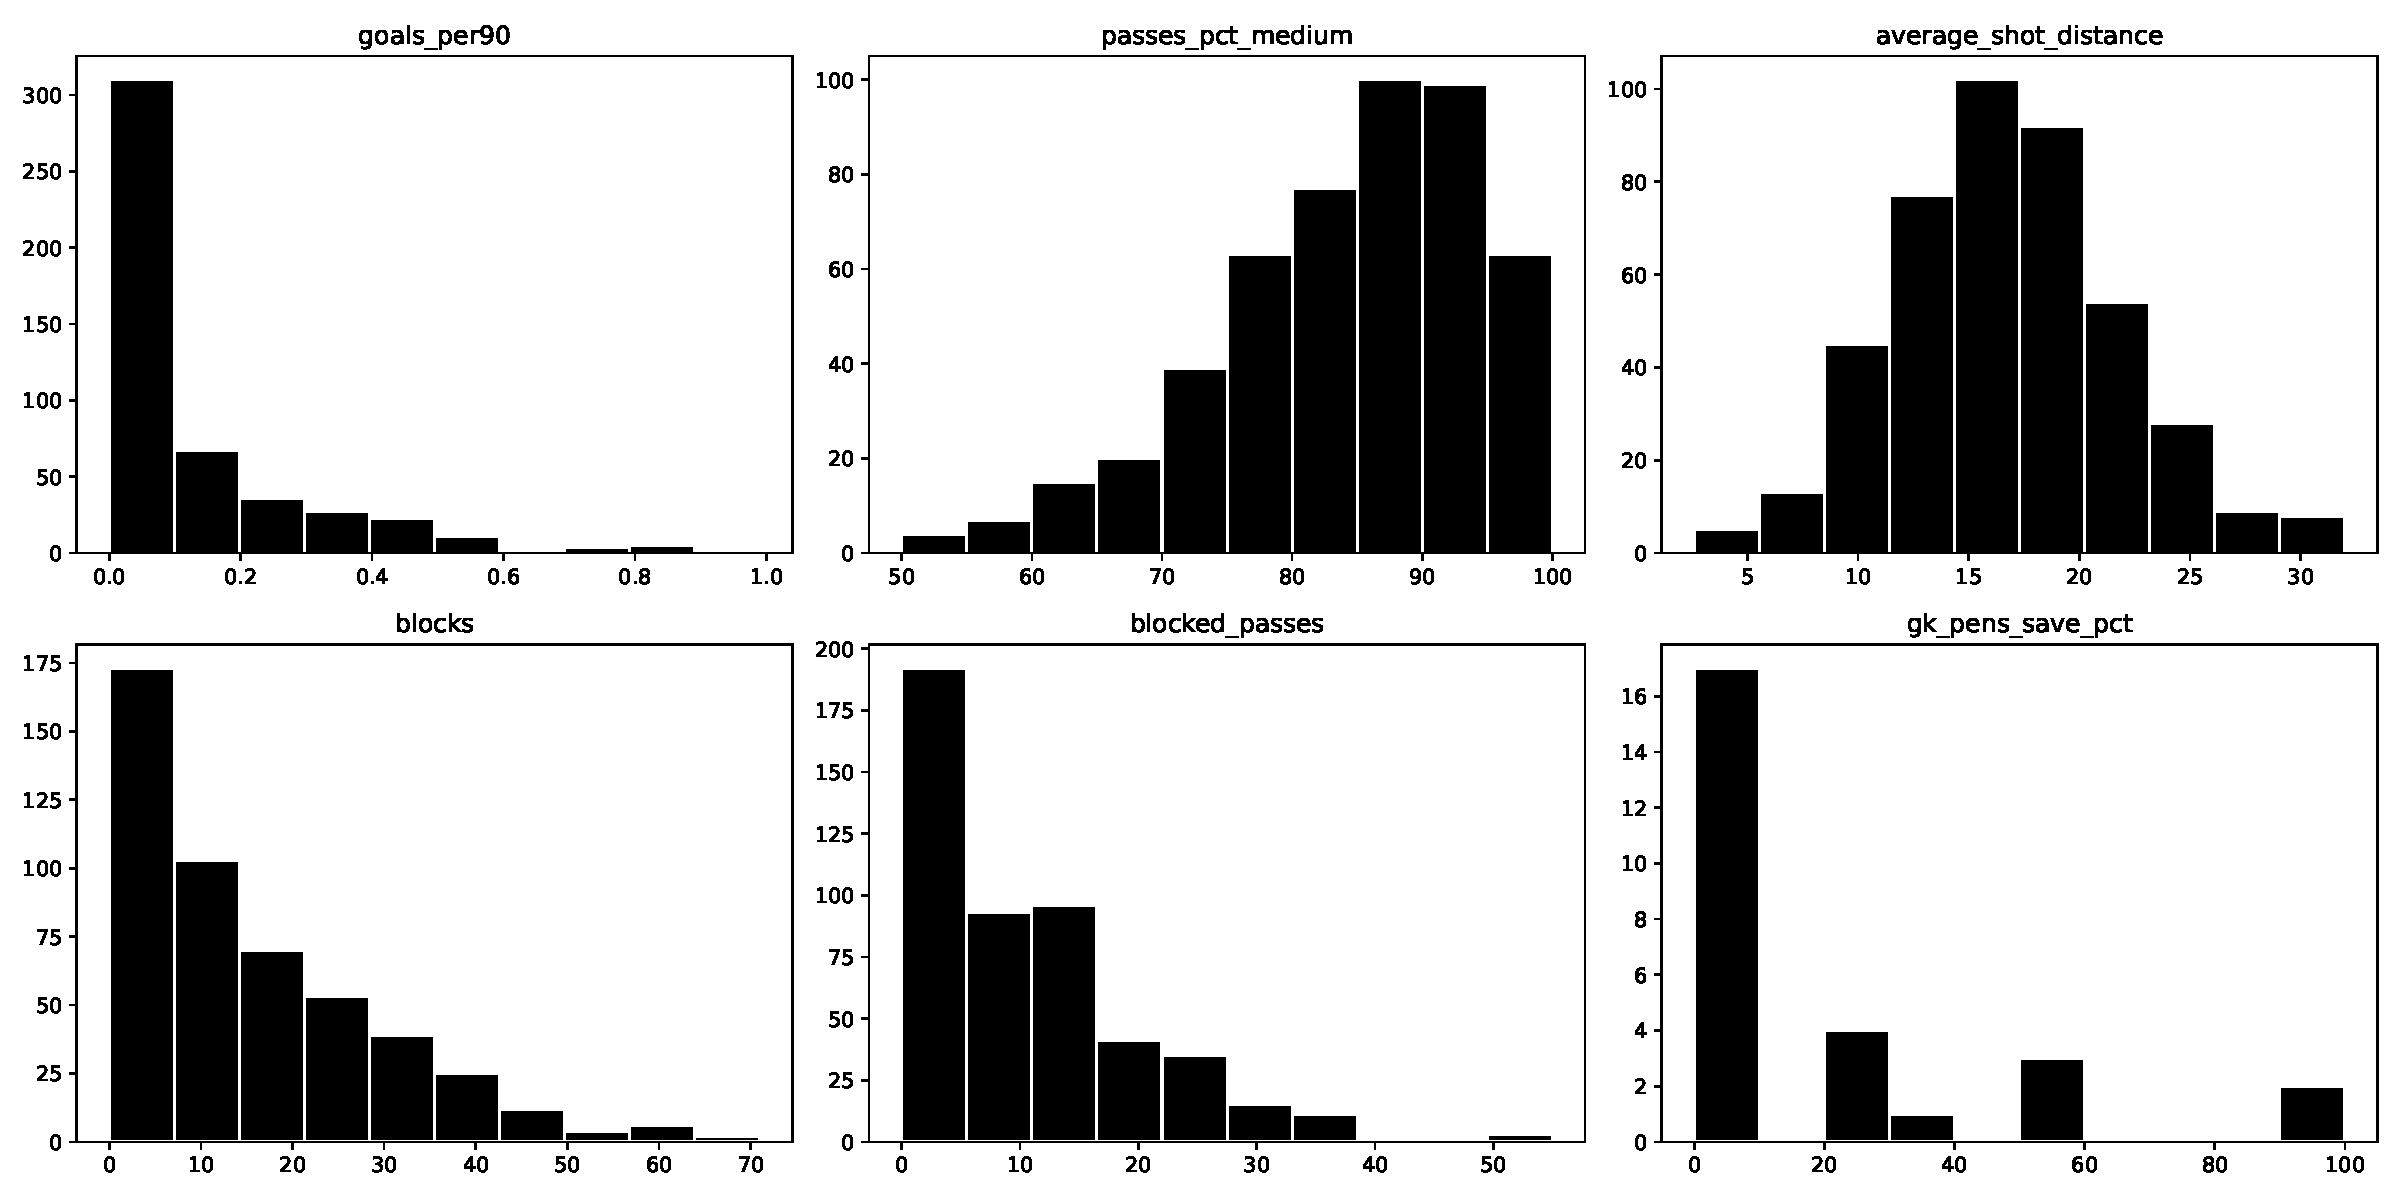
\includegraphics[width=\textwidth]{../output/task_ii/histograms/All.pdf}
    \caption{task\_ii/histograms/All.pdf}
\end{figure}

\newpage
\noindent
The Yeo-Johnson transformation is a power transform that can handle both positive and zero values, 
unlike Box-Cox (the transformation it is based on). This transformation would make the data more 
Gaussian-like (symmetrical).
\begin{verbatim}
    sklearn.preprocessing.power_transform(method='yeo-johnson')
\end{verbatim}
Yeo-Johnson Formula: 
\[ % had to chatgpt-ed this ngl
T(y; \lambda) =
\left\{
\begin{array}{ll}
\frac{(y + 1)^\lambda - 1}{\lambda}, & if y \geq 0,\ \lambda \ne 0 \\[6pt]
\log(y + 1), & if y \geq 0,\ \lambda = 0 \\[6pt]
- \frac{(-y + 1)^{2 - \lambda} - 1}{2 - \lambda}, & if y < 0,\ \lambda \ne 2 \\[6pt]
- \log(-y + 1), & if y < 0,\ \lambda = 2
\end{array}
\right.
\]
\begin{itemize}
    \item \( y \): the original data point.
    \item \( \lambda \): decides the transformation
    \item \( T(y; \lambda) \): the transformed value of \( y \).
\end{itemize}

\noindent
Finally, there are standardization and scaling.
\begin{verbatim}
    sklearn.preprocessing.StandardScaler().fit_transform()
\end{verbatim}
Euclidean distance is sensitive to feature scales. If one has an a large range, it can dominate the 
clustering result. This step makes sure that each statistic has a mean of 0 and a standard deviation 
of 1. The formula:
\[ X_{scaled} = \frac{X - Mean}{\textit{Standard Deviation}} \]

\subsubsection{Optimal K Clusters}
The method involves analyzing histograms of Inertia Elbow, Silhouette Score, Davies-Bouldin Index,
Calinski-Harabasz Index for a range of K from 2 to 20.
\begin{figure}[ht!]
    \centering
    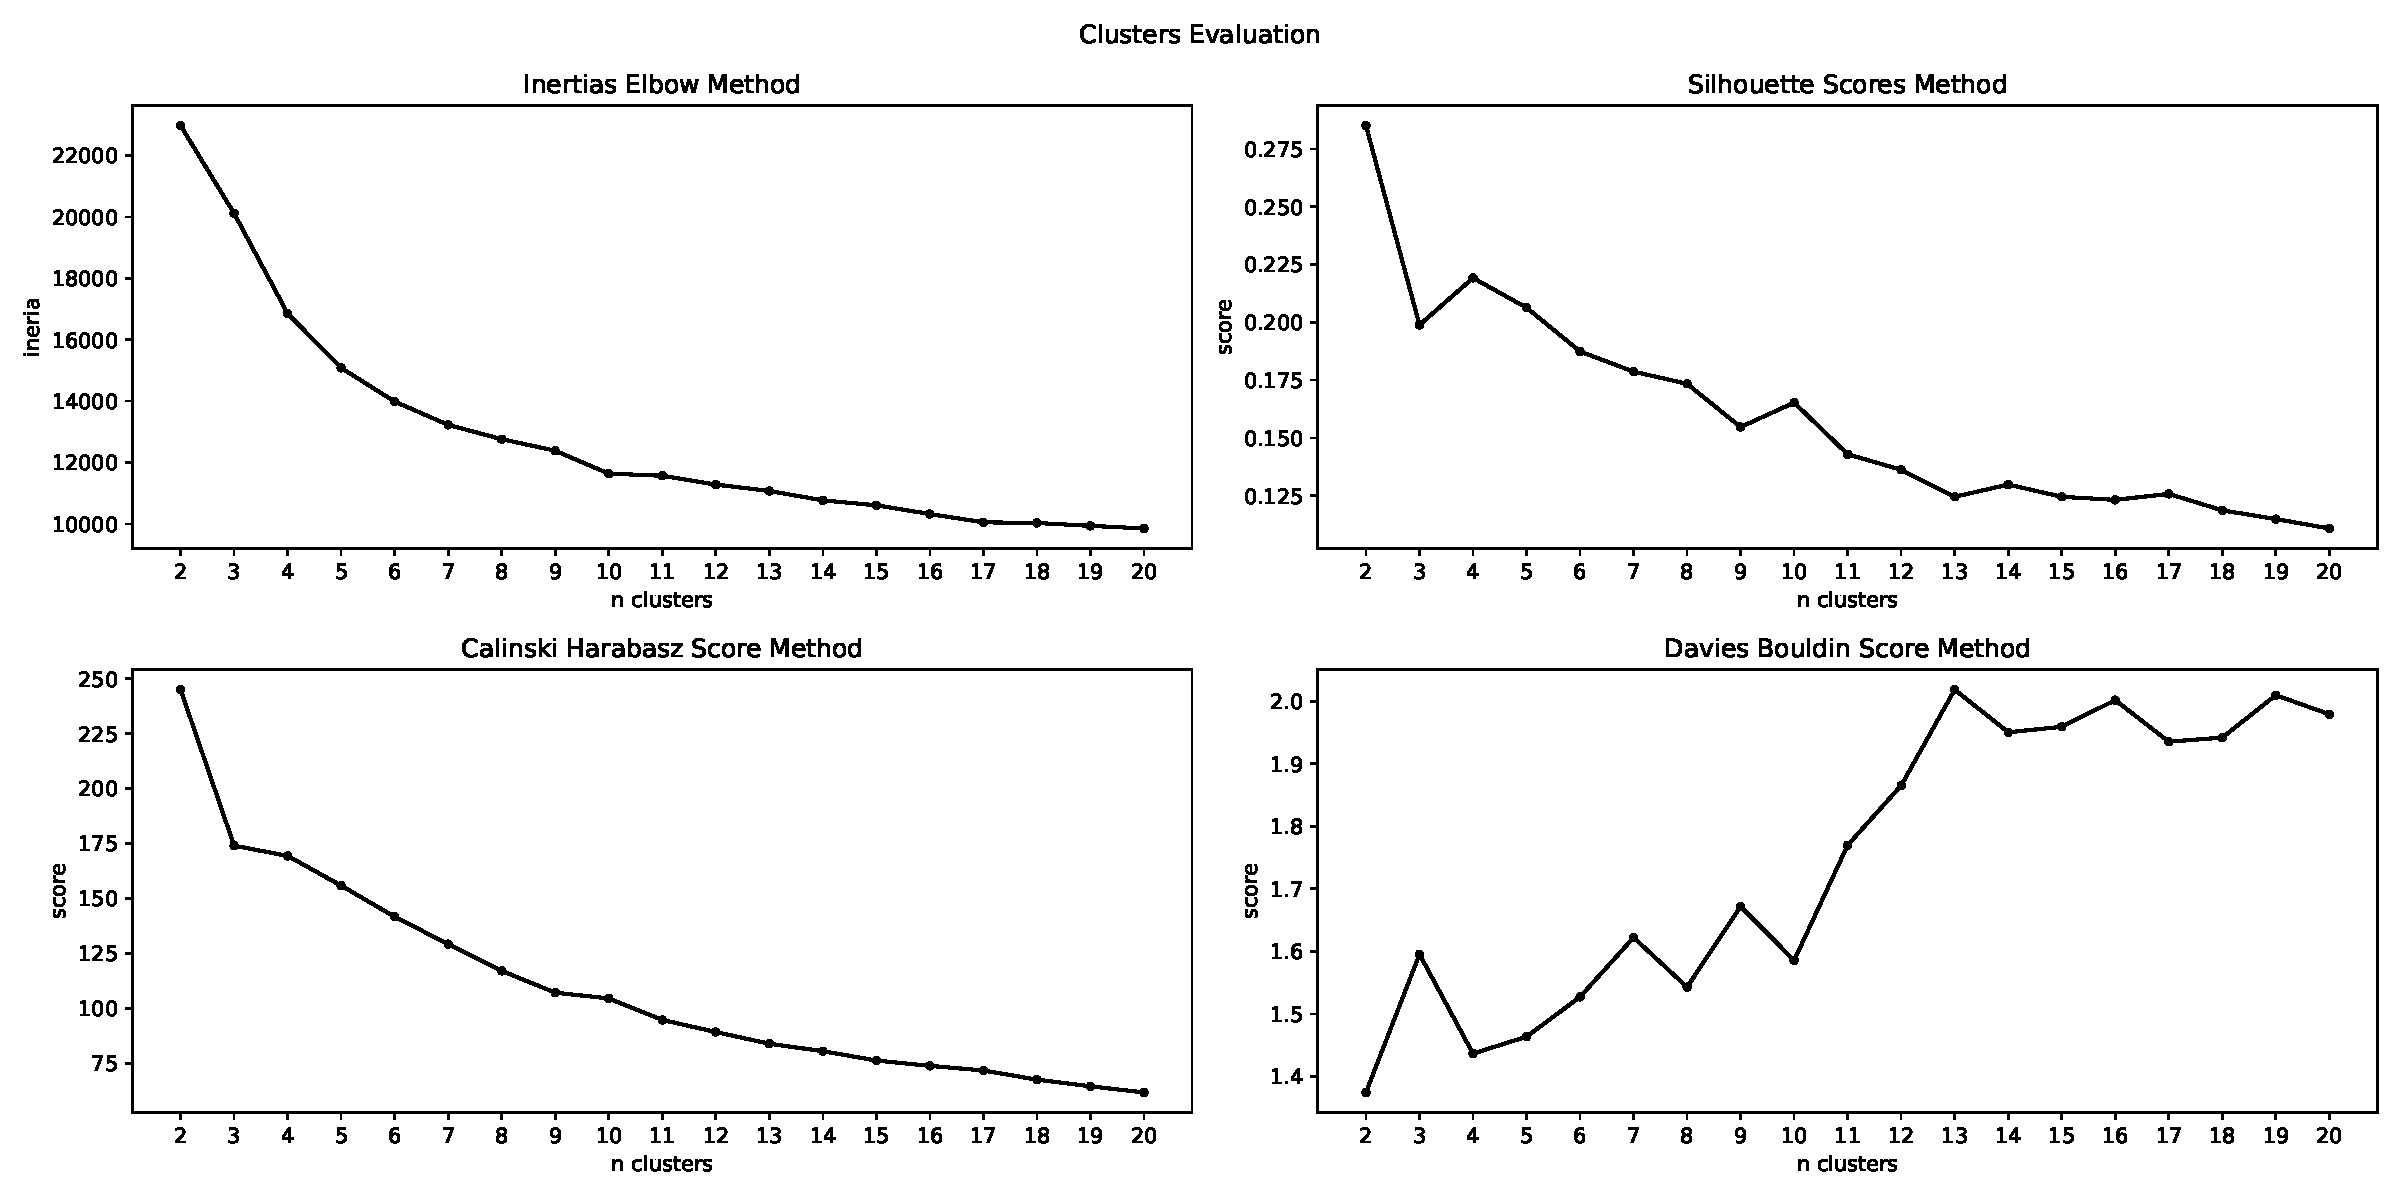
\includegraphics[width=\textwidth]{../output/task_iii/clusters_evaluation.pdf}
    \caption{task\_iii/clusters\_evaluation.pdf}
\end{figure}

\paragraph{Inertia Elbow:} measures how internally coherent the clusters are. A lower inertia 
indicates that the clusters are more compact and well-defined. But a higher K always result in a lower
Inertia, so it is best to pick $K_i$ where $K_{i+1}$ yields diminishing returns.
\[ Inertia_K = \sum_{i=1}^{N} \| x_i - c_i \|^2 \]
\begin{itemize}
    \item \( c_i \): Centroid of cluster i. 
    \item \( x \): Data Points of cluster i.
\end{itemize}

\paragraph{Silhouette Score:} measures how how similar each point is to its own cluster compared to 
other clusters. It ranges from -1 (worst) to +1 (best).
\[ Score_K = \frac{b(i) - a(i)}{\max\{a(i), b(i)\}} \]
\begin{itemize}
    \item \( a(i) \): average distance from point i to others points in the same cluster.
    \item \( b(i) \): average distance from point i to other points in other cluster.
\end{itemize}

\paragraph{Davies-Bouldin Index:}  evaluates the average similarity ratio of each cluster with the one 
most similar to it. The lower the better.
\[ DB_K = \frac{1}{K} \sum_{i=1}^{K} \max_{j \neq i} \left( \frac{S_i + S_j}{D(c_i, c_j)} \right) \]
\begin{itemize}
    \item \( S_i, S_j \): average distance from points to centroid of clusters i, j.
    \item \( D(c_i, c_j) \): Euclidean distance from centroids i to centroid j.
\end{itemize}

\paragraph{Calinski-Harabasz Index:}  evaluates the ratio of the sum of between-cluster dispersion to 
within-cluster dispersion. The higher the better.
\[ CH_K = \frac{tr(B_K)}{tr(W_K)} \cdot \frac{N - K}{K - 1} \]
\begin{itemize}
    \item \( tr(B_K) \): the between-cluster dispersion matrix.
    \item \( tr(W_K) \): the within-cluster dispersion matrix.
\end{itemize}

\noindent
Based on \verb|clusters_evaluation.svg|, K = 2 may looks good. But considering it may just be a 
goalkeepers cluster and an outfielders cluster, it is better to also split the outfielders into smaller
clusters. The actual K optimal chosen is 4.

\subsection{Principal Component Analysis (PCA)}
PCA is applied to reduce the dataset's dimensionality down to 2, allowing for a 2D scatter plot of data 
points. This visualization is the double checking if K = 4 is correct. The plot is saved to 
\verb|pca_clusters_2d.svg|.
\begin{verbatim}
    sklearn.decomposition.PCA(2).fit_transform()
\end{verbatim}
\begin{figure}[ht!]
    \centering
    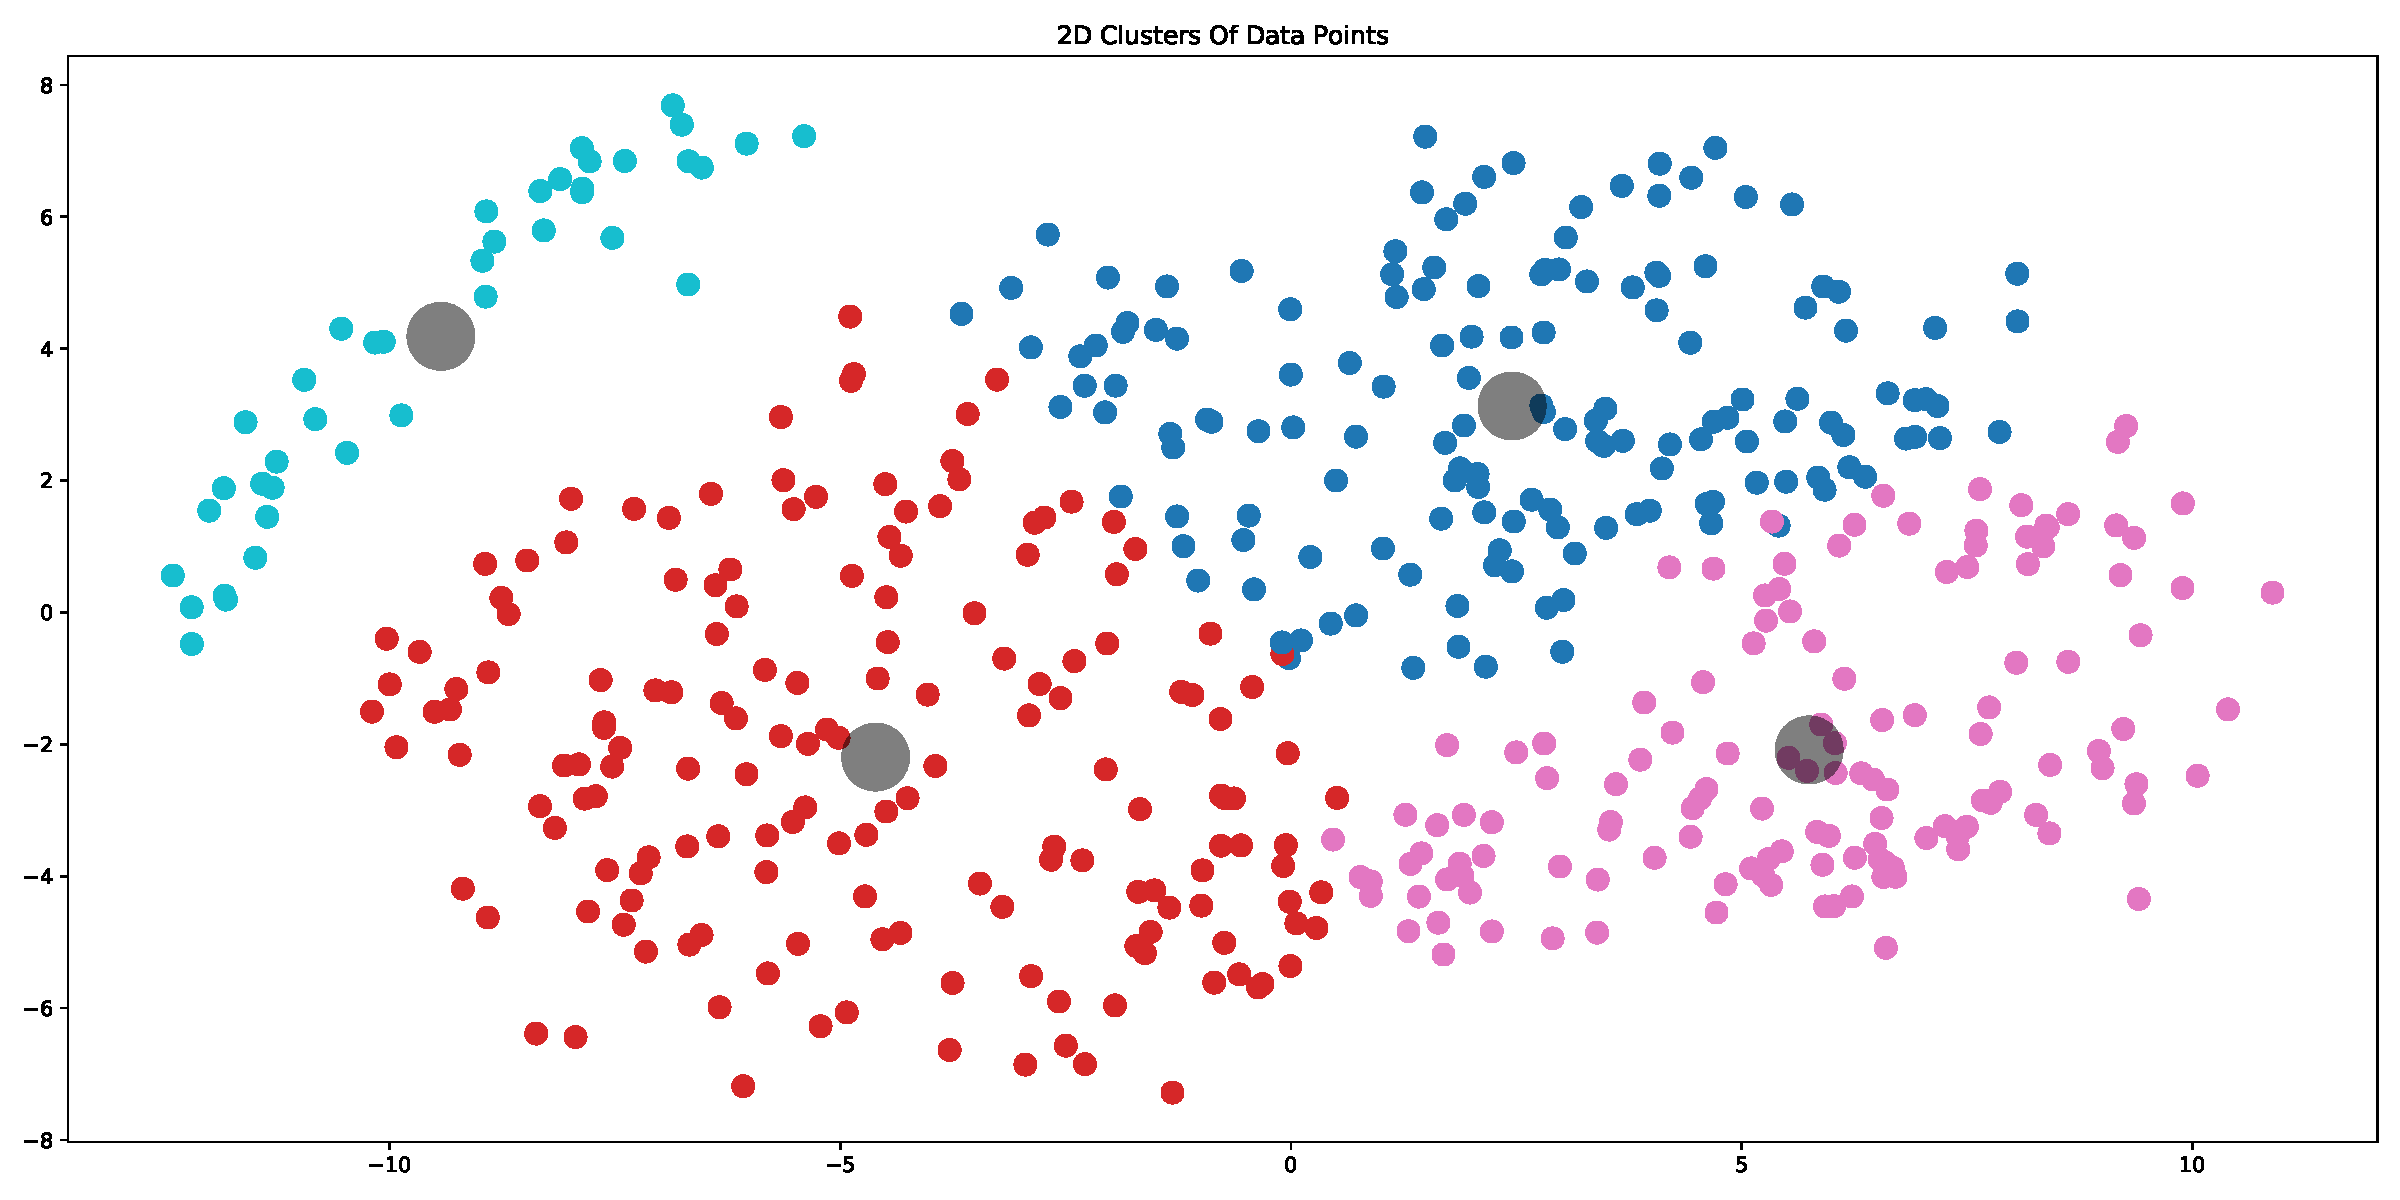
\includegraphics[width=\textwidth]{../output/task_iii/pca_clusters_2d.pdf}
    \caption{task\_iii/pca\_clusters\_2d.pdf}
\end{figure}
Analyzing the plot, the 4 clusters seems well seperated enough. Especially the top left cluster, which
most likely is the goalkeepers cluster.

\section{Task IV: Transfer Values Predicting}
Player transfer values are collected from \verb|footballtransfers.com| only for players with more than 
900 minutes of playing time. A proposed method for estimating the values involves:

\subsection{Identify The HTML Elements}
The task requires scraping transfer values from footballtransfers.com with playing time over 900 
minutes. The player names and minutes played data can be taken from task I. Unlike fbref.com 
source which is static HTML, footballtransfers.com loads its content dynamically using JavaScript.
\begin{verbatim}
    <|-- Table Before JavaScript Loaded -->
    <tbody id="player-table-body">
        <tr class="table-placeholder">
            <!-- empty td -->

    <|-- Table After JavaScript Loaded -->
    <tbody id="player-table-body">
        <tr>
            <td class="td-player">
                <span>
                    Erling Haaland
                <\span>
            <\td>
            <td class="text-center">
                <span>
                    €198.8M
                <\span>
        <!-- other tr -->
\end{verbatim}

\noindent
Therefore, selenium need to wait before the table gets fully loaded.
\begin{verbatim}
    WebDriverWait(driver, 30).until(
        EC.presence_of_element_located((
            By.CSS_SELECTOR, 
            "tbody#player-table-body > tr:not(.table-placeholder)"
        ))
    )
\end{verbatim}

\noindent
The simply point CSS selector to the name and transfer value of the player which has played
above 900 minutes.
\begin{verbatim}
    tbody#player-table-body > tr            /* target all tr */
    tr > td.td-player > span                /* target name */
    tr > td.text-center > span              /* target transfer value */ 
\end{verbatim}

\subsection{Training Model}
This section can be split into three main parts:
\begin{itemize}
    \item \textbf{Choosing a linear model}: output files include \verb|pca_2d.svg|
    \item \textbf{Prepare Dataset} 
    \item \textbf{Performing Tests}: output files include \verb|bootstrapping_scores.svg|,
    \item \textbf{Result}: output files include \verb|feature_importance.svg|, 
    \verb|transfer_values_predicted.csv|
\end{itemize}

\subsubsection{Choosing a linear model}
Estimated transfer values of a players are often influenced by that players statistics. The higher
the stats, the higher the transfer value. \verb|pca_2d.svg| shows that, despites not having done
features selection, the plot still resembles a clear linear pattern. \\
\begin{figure}[ht!]
    \centering
    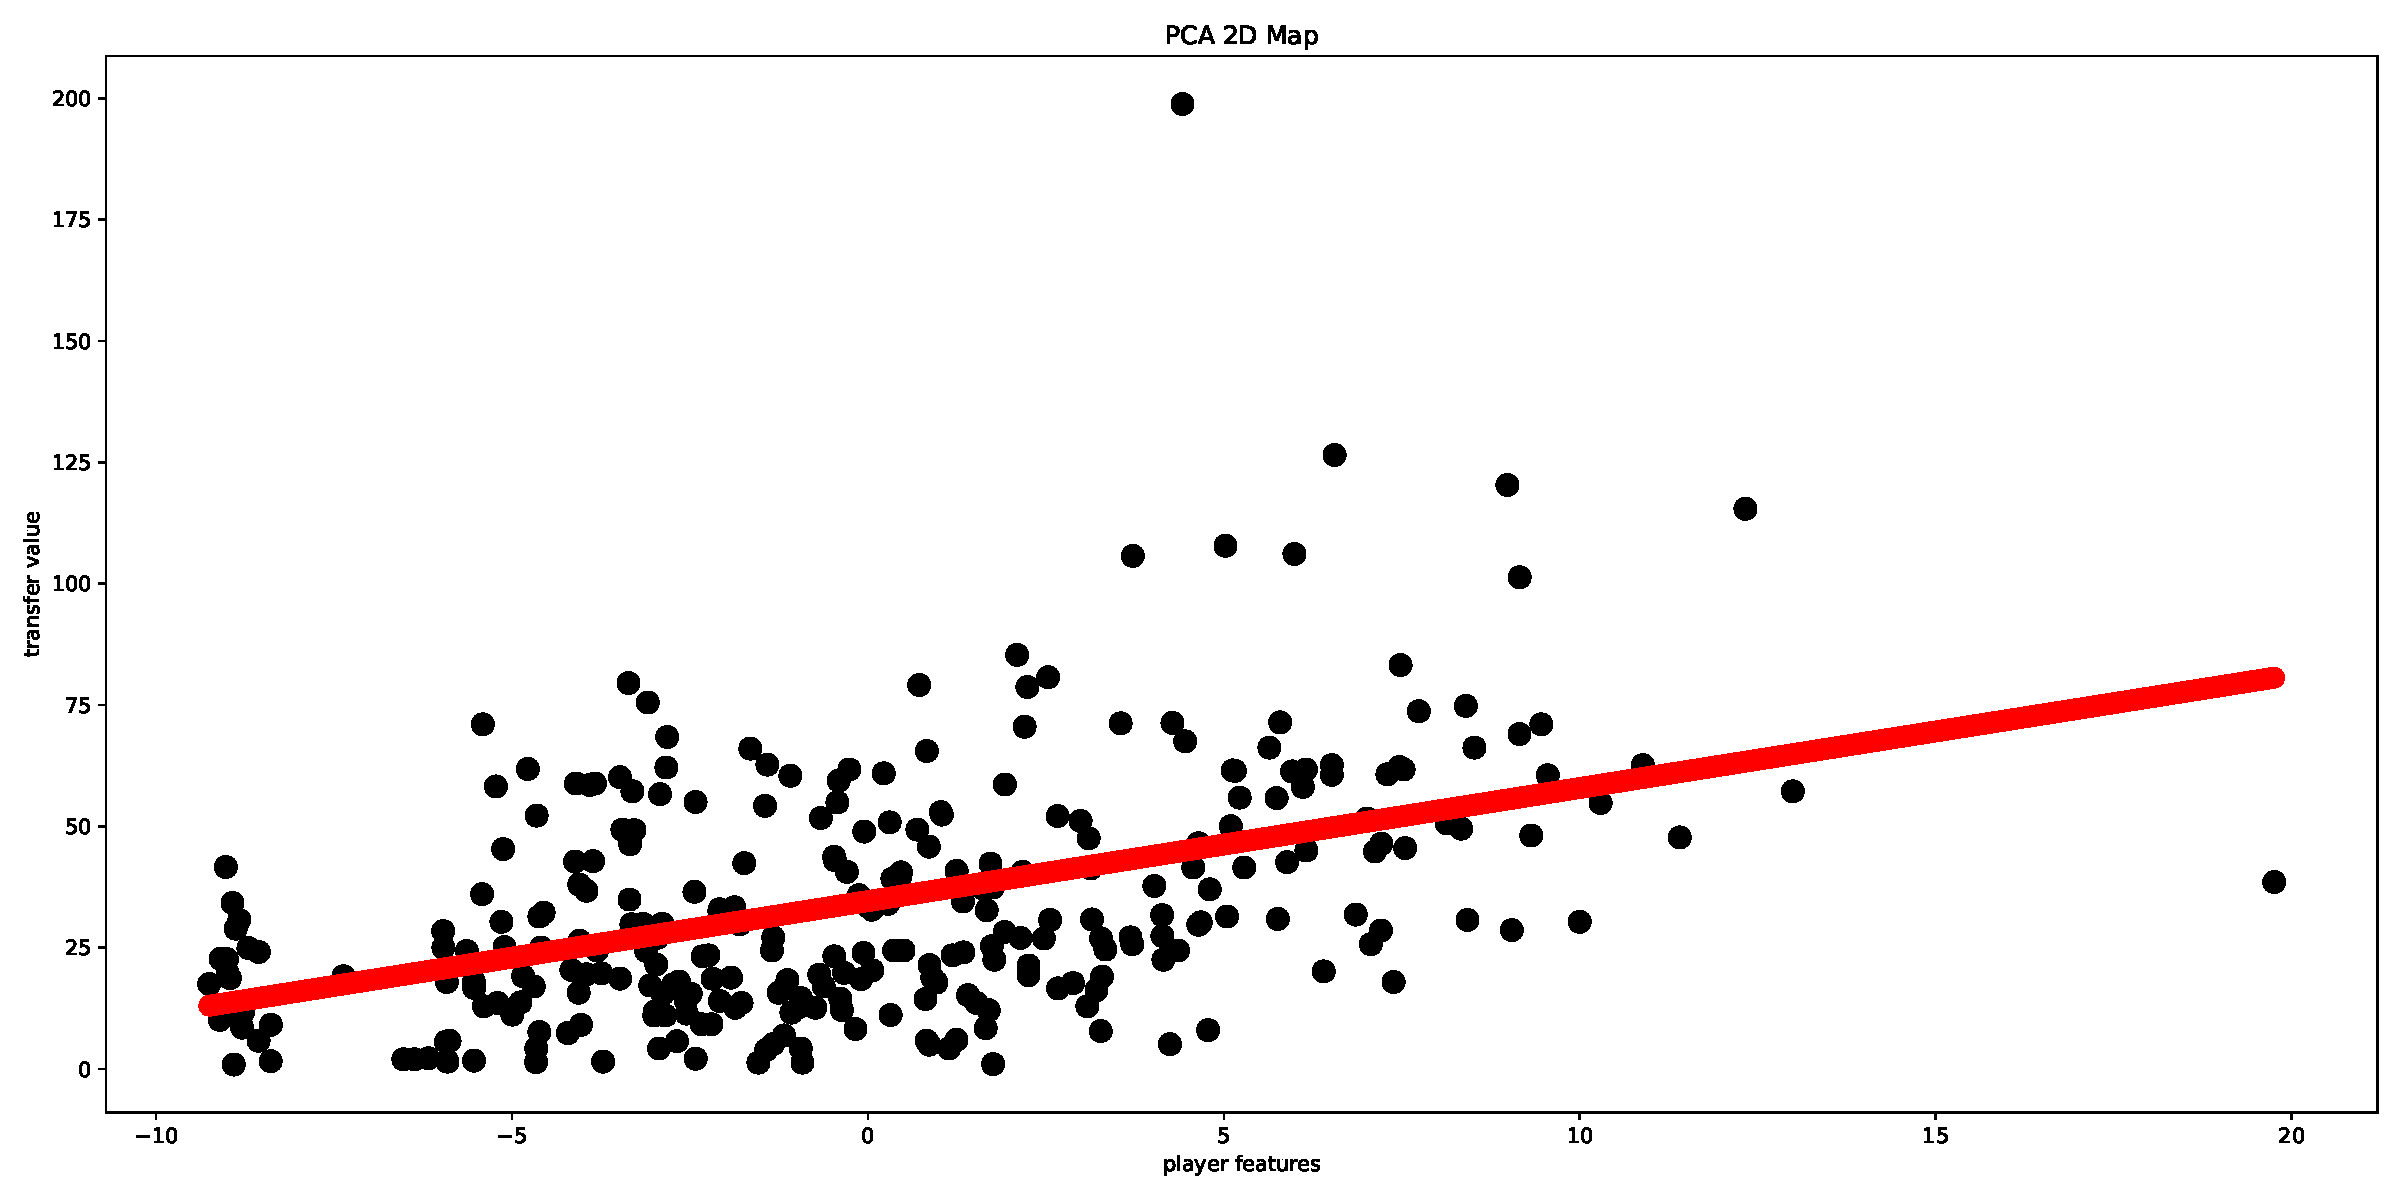
\includegraphics[width=\textwidth]{../output/task_iv/pca_2d.pdf}
    \caption{task\_iv/pca\_2d.pdf}
\end{figure}

\newpage
\noindent
If the criterias are being easy to implement, fast training and decent performace, then 
Linear Model is a perfect fit. More specifically, LassoCV model. \\

\noindent
Lasso can perform both regression and automatic feature selection. By adding an L1 penalty, 
it can decrease non important features coefficients to zero. \\

\noindent
The difference between Lasso and LassoCV is that LassoCV use cross-validation to 
automatically select the optimal alpha parameter. Making LassoCV easy to use while still being 
performant. \\

\noindent
Lasso Regression Objective Function:
\[  % no shot I made this
    \hat{\beta} = \arg\min_{\beta} \left\{ \frac{1}{2n} \sum_{i=1}^{n} 
    (y_i - X_i^{\top} \beta)^2 + \alpha \sum_{j=1}^{p} |\beta_j| \right\}
\]
\begin{itemize}
    \item \( n \): samples count
    \item \( p \): features count
    \item \( X_i \): feature vector for sample i
    \item \( y_i \): target value for sample i
    \item \( \beta \): vector of regression coefficients
    \item \( \alpha \): regularization parameter (L1 penalty strength)
\end{itemize}

LassoCV selecting $\alpha$ using cross-validation:
\[ \alpha^* = \arg\min_{\alpha} CVError(\alpha) \]
\begin{itemize}
    \item \( CVError \): average cross-validated prediction error for each tested value
\end{itemize}

\subsubsection{Prepare Dataset}
Handling missing value N/a is the same as task III. \\

\noindent
For this case, the dataset can be One-Hot encoded. \\
One-Hot Encoding is the technique to transform each categorical features values into individuals
binary columns. For each categorical feature encoded, a column is dropped to prevent multicollinearity,
which is important for linear models like Lasso. \\
Even though, the number of features would increases significantly, the non important ones can 
be dropped later during features selection. \\ 
Unlike other linear models, Lasso is sensitive to feature scales because it penalizes coefficients via 
L1 regularization. Therefore scaling and standardization are still applied.  

\subsubsection{Performing Tests}
To assess the stability and reliability of the model, bootstrapping was selected. Bootstrapping is a 
resampling technique on the dataset to output N new random samples for scoring. This makes sure that 
the scores was not just a fluke. \\
\begin{verbatim}
    # pseudocode
    def bootstrap(data, model, num_samples):
    scores = []
    
    for i in range(num_samples)
        bootstrap_sample = draw_bootstrap_sample(data)
        model.fit(bootstrap_sample)
        score = model.evaluate(data)
        scores.append(score)
    
    average_score = average(scores)
    return average_score
\end{verbatim}

\noindent
R2 Score and RMSE are used for evaluating the model.
\[ R^2 = 1 - \frac{\sum_{i=1}^{N} (y_i - \hat{y}_i)^2}{\sum_{i=1}^{N} (y_i - \bar{y})^2} \]
\[ RMSE = \sqrt{\frac{1}{N} \sum_{i=1}^{N} (y_i - \hat{y}_i)^2} \]
\begin{itemize}
    \item \( y \): the true target values.
    \item \( \hat{y} \): the predicted target values.
    \item \( \bar{y} \): the mean of the true target values.
\end{itemize}

\noindent
Since a high sample counts would take longer time, number of samples = 10 was settled on in the program.
\verb|bootstrapping_scores.svg| shows that R2 Score average around 0.7, RMSE is around 14.0. An 
acceptable result.
\begin{figure}[ht!]
    \centering
    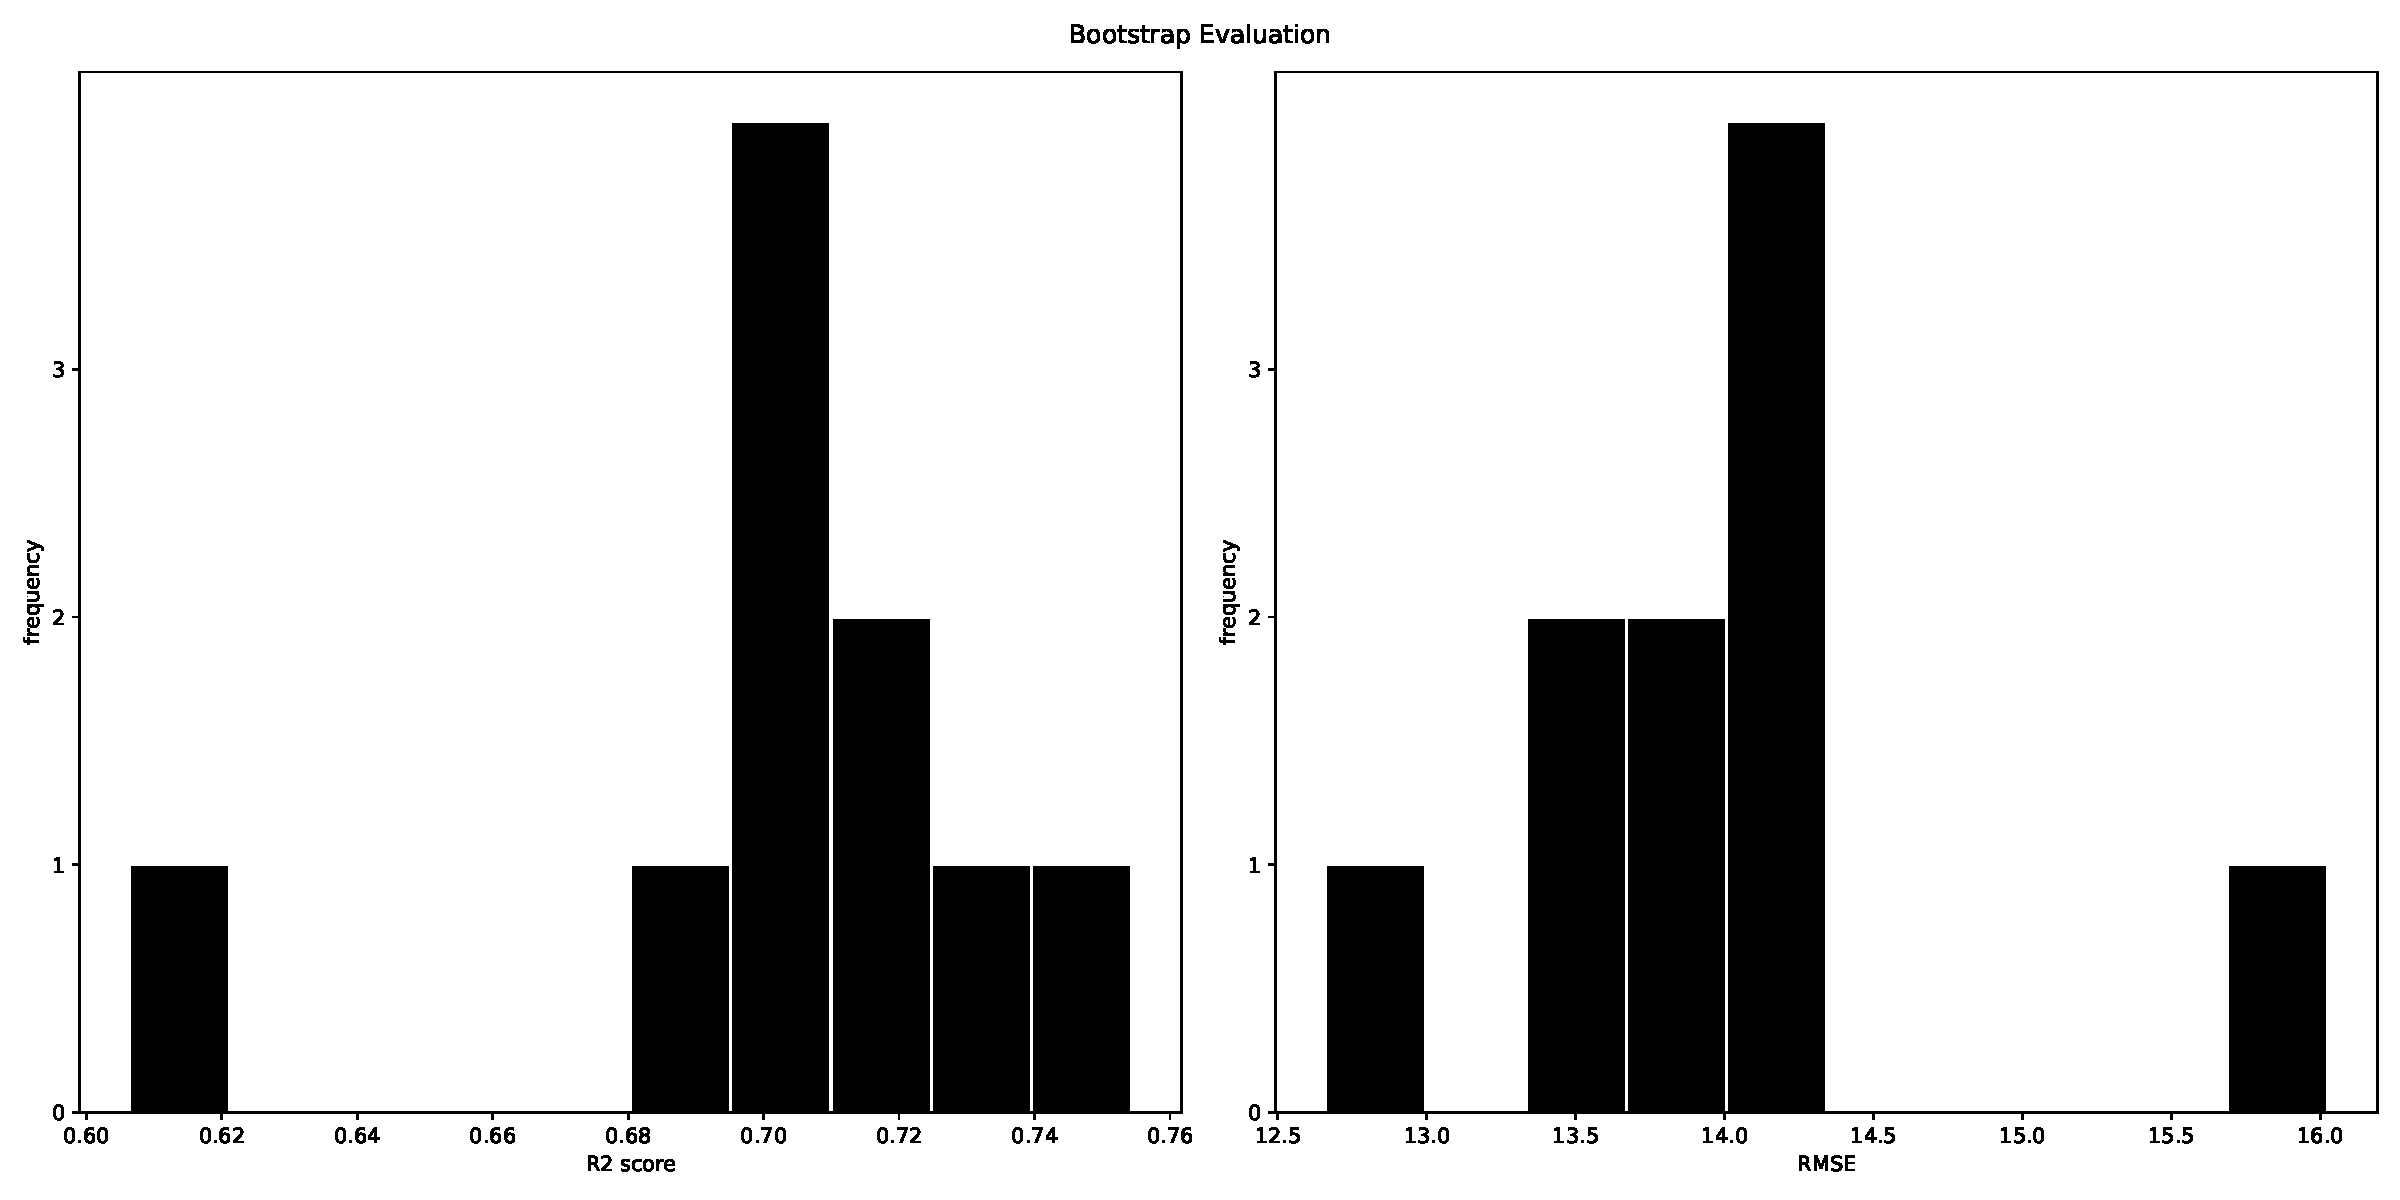
\includegraphics[width=\textwidth]{../output/task_iv/bootstrapping_scores.pdf}
    \caption{task\_iv/bootstrapping\_scores.pdf}
\end{figure}

\newpage
\subsubsection{Result}
Analyzing \verb|transfer_values_predicted.csv|, some of the model's predictions are quite close to
the true value, while some are off by a whole landslide. Especially the ones with negative values. 
Brutal. \\
\verb|feature_importance.svg| shows some interesting insights. Age is the most deciding factor, and
by a lot. The team and nationality statistics also ranks very high up on the graph. Performance 
statistics appear less than expected, which can be explained by the fact that those may be correlated 
with each other, leading to LassoCV dropping them.
\begin{figure}[ht!]
    \centering
    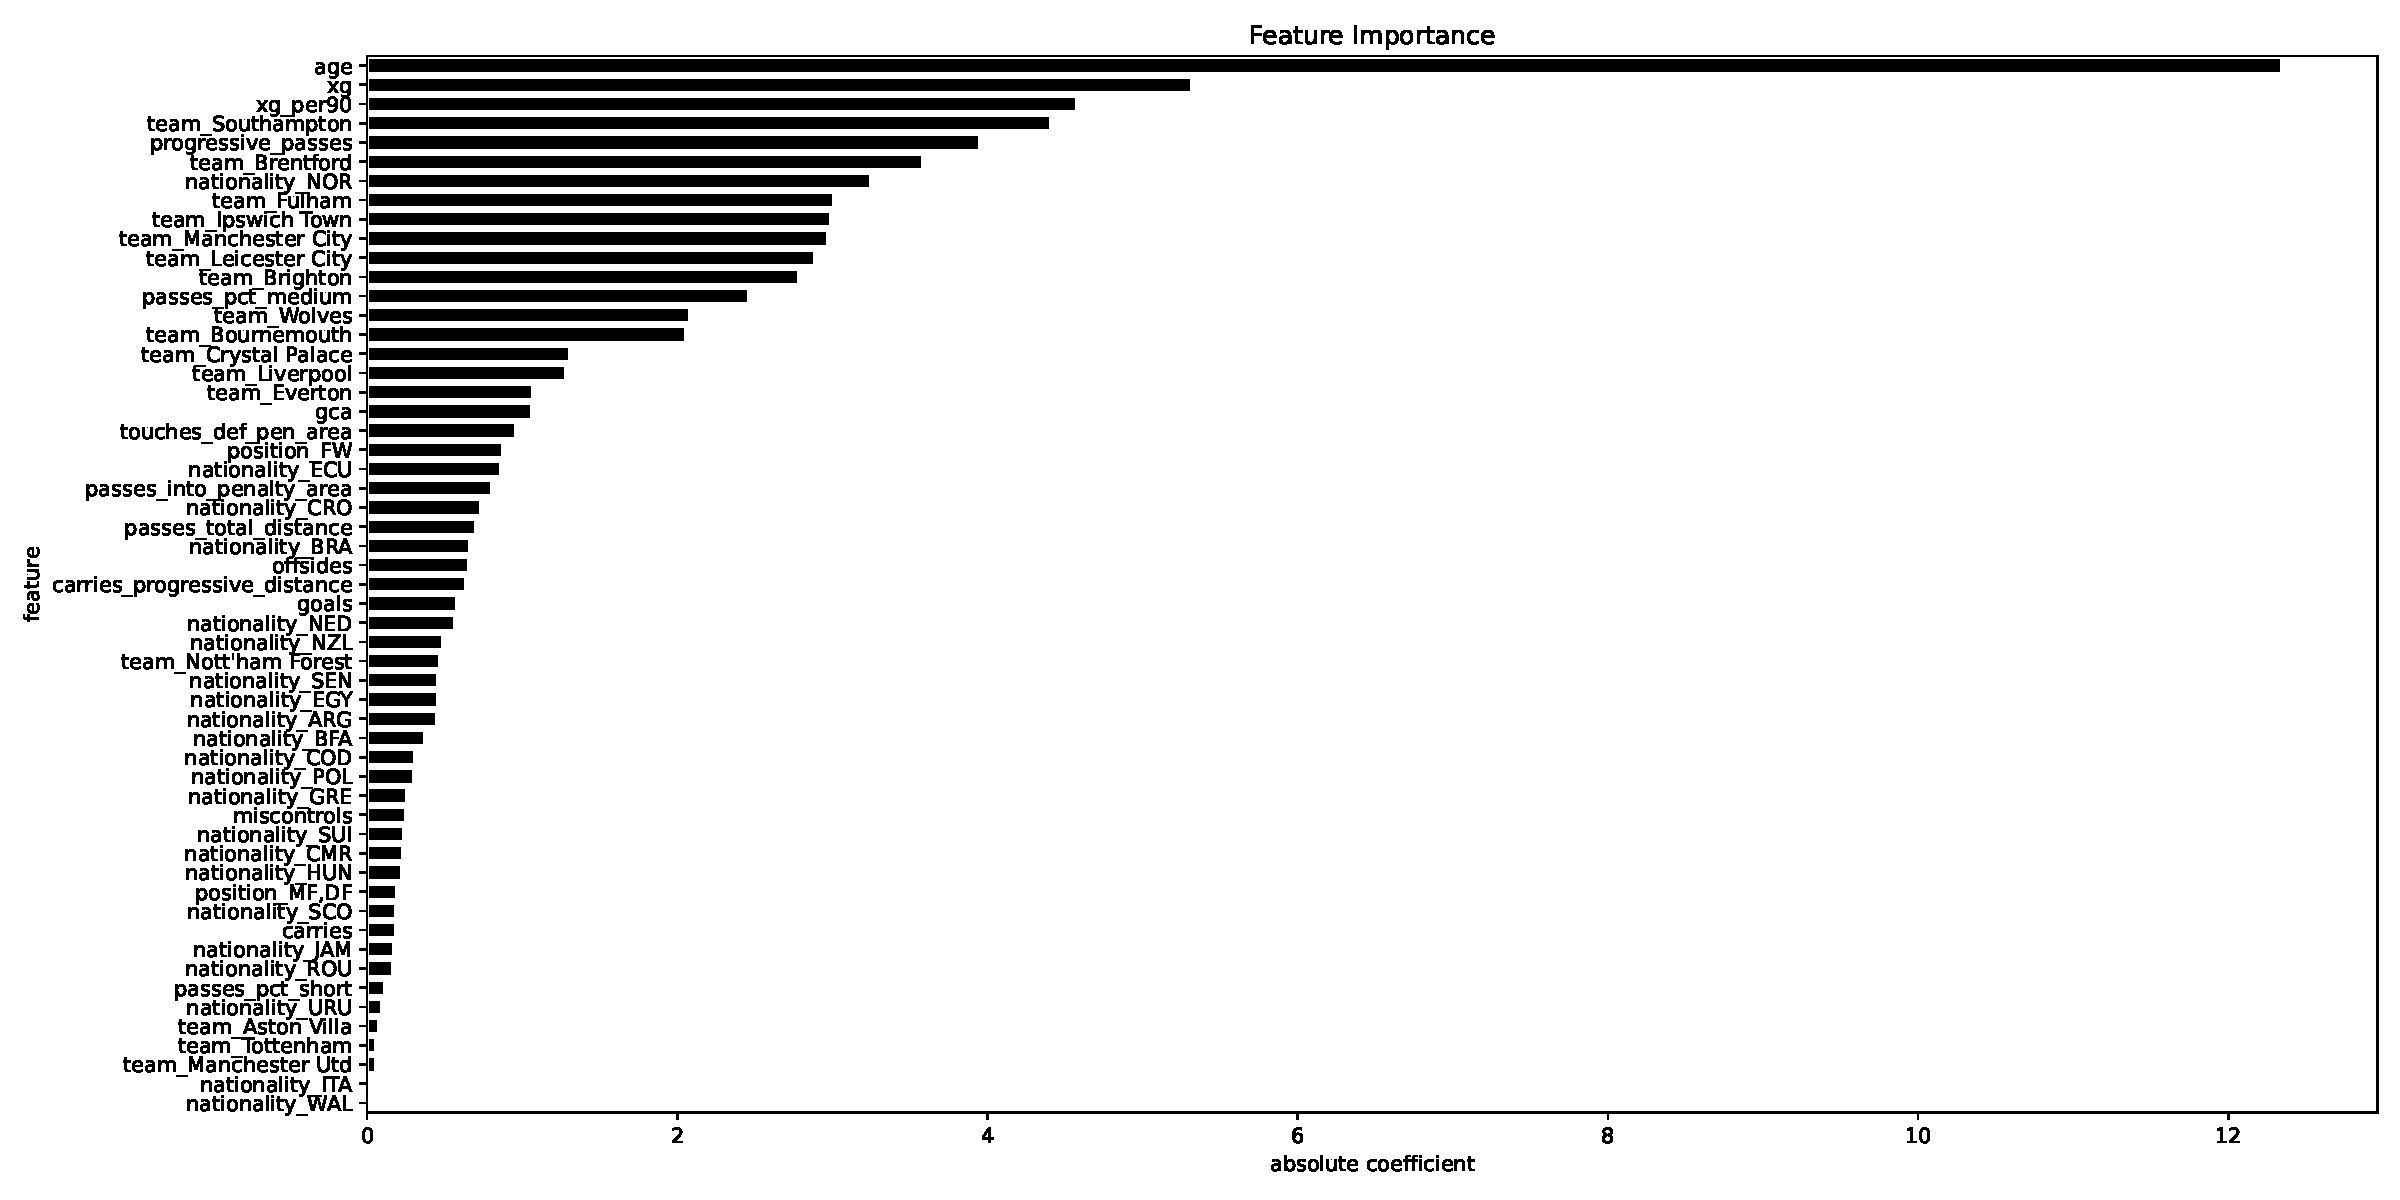
\includegraphics[width=\textwidth]{../output/task_iv/feature_importance.pdf}
    \caption{task\_iv/feature\_importance.pdf}
\end{figure}

\section{Conclusion}
Overall, this report reviews and explains the entire process of data collection, analysis, clustering, and 
transfer value predicting using data from \verb|fbref.com| and \verb|footballtransfers.com|. 
The assignment was a great way to study and understand Data Science and Machine Learning. \\

\textbf{Reference documents}: \\
{\small \verb|https://s3.amazonaws.com/assets.datacamp.com/production/course_10628/slides/chapter3.pdf|} \\
{\small \verb|https://www.geeksforgeeks.org/powertransformer-in-scikit-learn|} \\ 
{\small \verb|https://www.geeksforgeeks.org/feature-encoding-techniques-machine-learning|} \\
{\small \verb|https://www.geeksforgeeks.org/cross-validation-vs-bootstrapping|} \\
{\small \verb|https://www.youtube.com/watch?v=d6iQrh2TK98|} \\

% Isn't this where...

\end{document}
